A implementação do algoritmo de criptografia foi centralizada por meio de uma classe, de forma que o cálculo dos valores relacionados às chaves fosse mais acessível e didático. É possível configurar tanto o método de teste de primalidade (força bruta, Fermat ou Miller-Rabin) quando o tamanho dos bits a serem utilizados.

Após a geração dos valores $p$ e $q$ o método \texttt{generate-keypair} realiza o cálculo dos valores $n$ e $\phi(n)$, assim como a definição do valor $e$ e cálculo do $d$, utilizados nas chaves pública e privada, respectivamente.

A criptografia em si consiste no recebimento de uma mensagem e da chave pública $(e,n)$, aplicadas na fórmula $c = m^e mod n$  considerando o código da tabela ASCII de cada caracter individualmente, o que é posteriormente salvo em um arquivo texto para consulta.

A descriptografia, por sua vez, realiza o procedimento inverso pela leitura do arquivo com o texto criptografado e aplicação do valor de cada caracter na fórmula $m = c^d mod n$, obtendo o valor original.


Para análise do tempo de execução foram realizadas combinações de algoritmos, contemplando diferentes processos para execução do teste de primalidade. A metodologia para coleta de dados consistiu na execução do processo de criptografia por 10 vezes consecutivas, com a exclusão das medições de menor e de maior valor. A implementação foi configurada para utilizar tamanhos de palavras variadas, de 4 em 4 bits até 32 bits. A Tabela~\ref{tab:encryptTable} demonstra a diferença de tempo para geração das chaves utilizando os algoritmos de primalidade por força bruta,Miller-Rabin e Fermat.

\begin{table}[!htbp]
\centering
\caption{Tempo de geração das chaves (em segundos) \textit{x} Número de Bits.}
\label{tab:encryptTable}
\begin{tabular}{|l|l|l|l|}
\hline
\textbf{Bits} & \textbf{Prime} & \textbf{Miller} & \textbf{Fermat} \\ \hline
\textbf{4} & 0.1035 & 0.0002 & 0.0005 \\ \hline
\textbf{8} & 0.2942 & 0.0002 & 0.0005 \\ \hline
\textbf{16} & 1.0023 & 0.0007 & 0.0007 \\ \hline
\textbf{24} & 6.9885 & 0.0004 & 0.0022 \\ \hline
\textbf{32} & 824.30 & 0.0013 & 0.0045 \\ \hline
\end{tabular}
\end{table}


É possível notar uma grande diferença de tempo entre o modelo de força bruta e a aplicação dos algoritmos Miller-Rabin e Fermat, o que se torna ainda mais evidente quando se aumenta o tamanho da chave. A melhor performance resultante dos testes foi do Algoritmo de Miller-Rabin, o que justifica ser o teste mais utilizado nas soluções de criptografia e um dos mais eficientes da atualidade \cite{ribeiro:2014}. No gráfico a seguir é possível visualizar as linhas que representam a complexidade de tempo exponencial para o algoritmo de força bruta (prime), em relação com o crescimento logarítmico dos algoritmos Miller-Rabin e Fermat. % (Dietzfelbinger 2004)

\begin{figure}[!htbp]
\centering
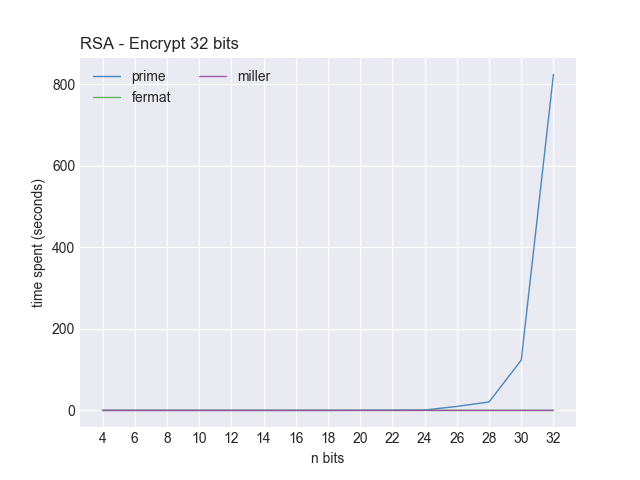
\includegraphics[width=0.75\textwidth]{images/32_Encrypt.png}
\caption{Tempo de geração das chaves (em segundos) \textit{x} Número de Bits.}
\label{fig:encryptFig}
\end{figure}
